\documentclass{article}
\usepackage[utf8]{inputenc}

\usepackage{amsmath}
\usepackage{amssymb}
\usepackage{siunitx}
\sisetup{range-phrase=--}
\sisetup{range-units=single}
\sisetup{per-mode=symbol}

\usepackage{xcolor}
\usepackage[unicode]{hyperref}
\usepackage{minted}
\usepackage{fullpage}

\usepackage{tikz}
\usepackage[siunitx]{circuitikz}

\usepackage{enumitem}

\usepackage{import}

\newcommand{\mat}[1]{\left[\begin{matrix}#1\end{matrix}\right]}
\newcommand{\vectwo}[2]{\left[\begin{matrix}#1\\#2\end{matrix}\right]}
\newcommand{\mattwo}[4]{\left[\begin{matrix}#1 & #3\\#2 & #4\end{matrix}\right]}

\DeclareMathOperator{\dive}{div}
\DeclareMathOperator{\grad}{grad}
\DeclareMathOperator{\tr}{tr}

\title{MECH3780}
\author{MECH3780 team}

\newcommand{\rr}[2]{\frac{\partial #1}{\partial #2}}
\newcommand{\pr}[1]{\frac{\partial}{\partial #1}}

\AddToHook{cmd/section/before}{\clearpage}
\AddToHook{cmd/subsection*/before}{\clearpage}
\newtheorem{exercise}{Exercise}[section]

\begin{document}
\maketitle
\section{Lecture}
\subsection{Course (and software) introduction}
Chris explaining what a book is, and how to use it.
\subsection{The computational analysis workflow}
Explaining that most computational engineering analysis will consist of:
\begin{itemize}
\item Preparation of geometry --- in which you recreate the geometry of interest
\item Meshing --- in which you divide the domain of interest into small pieces called elements
\item Simulation setup --- in which you define what physical phenomena you want to simulate and what material properties you want to use
\item Computation --- in which you use a high-efficiency hardware to solve the posed numerical problem
\item Post-processing and analysis --- in which you analyse the results, but also check if your meshing and setup allowed for accurate solution of the physical problem
\item Design improvement --- in which you use the constructed workflow to iterativelly improve the performance of the considered design.
\end{itemize}
\subsection{Introduction to the FEM}
Derivation of force balance in a sprint under tension.

From Hook's law:
\[F = kx\]
Calculating balance on two end points:
\[\begin{cases}
    F_0 + (x_1 - x_0)k &= 0\\
    F_1 - (x_1 - x_0)k &= 0
\end{cases}\]
In matrix form:
\[\mattwo{k}{-k}{-k}{k}\vectwo{x_0}{x_1}=\vectwo{F_0}{F_1}\]

Show a system of springs,
\begin{center}
\begin{circuitikz}
\draw 
(0,0) to[R={$k_2$},*-*] (5,1) to[R={$k_1$},-*] (8,0)
(0,0) to[R={$k_1$},-*] (3,-1) to[R={$k_2$},-] (8,0)
(3,-1) to[R={$k_3$},-] (5,1);
\draw [->,dashed] (0,0) |- (1,-1.5);
\draw [->,dashed] (3,-1) |- (4,-1.5);
\draw [->,dashed] (5,1) |- (6,-1.5);
\draw [->,dashed] (8,0) |- (9,-1.5);
\end{circuitikz}
\end{center}

and show how they contribute to a bigger matrix:
\[\mat{
k_1+k_2 & -k_1 & -k_2 & 0\\
-k_1 & k_1+k_2+k_3 & -k_3 & -k_2\\
-k_2 & -k_3 & k_1+k_2+k_3 & -k_1\\
0 & -k_2 & -k_1 & k_1+k_2}\mat{x_0\\x_1\\x_2\\x_3} = \mat{F_0\\F_1\\F_2\\F_3}\]
What are the element degrees of freedom and global degrees of freedom. Define what is an element matrix and what is the global stiffness matrix.

But in most cases, we have the forces and we want to compute the displacements. But the matrix is (obviously) degenerate [insert a rumbling side-note about the fact that matrix invertability is equivalent with a empty null space, and tying null spaces to invariance and fixing structural degrees of freedom).

How to introduce fixed-displacement boundary conditions:
\[\mat{
1 & 0 & 0 & 0\\
-k_1 & k_1+k_2+k_3 & -k_3 & -k_2\\
-k_2 & -k_3 & k_1+k_2+k_3 & -k_1\\
0 & -k_2 & -k_1 & k_1+k_2}\mat{x_0\\x_1\\x_2\\x_3} = \mat{d_0\\F_1\\F_2\\F_3}\]

Energy interpretation of the FEM. Potential energy of a spring $\frac{1}{2}kx^2$, and work $Fx$. Same expressions become matrix expressions $\frac{1}{2}x^TSx$ and $F^Tx$ respectively. Potential energy of complex element (as in contrast to springs) can sometimes be easier derived than literal expressions for forces. Moreover this interpretation allows for more complex force distributions and generalised degrees of freedom.

\subsection{Direct method of derivation for a beam/truss}

Example of a beam at and angle. Expression for energy:
\[\frac{1}{2}\frac{AE}{L}(x\cdot n)^2\]
where $A$, $E$ and $L$ are cross-section area, Young modulus and length of the beam respectively. And $n$ is the vector in the direction of the beam. And work is simply $F\cdot x$. From that we can derive:
\begin{align*}\frac{1}{2}\underbrace{\frac{AE}{L}}_k((x_1-x_0)\cdot n)^2 &= \frac{1}{2}k(x^x_1n_x+x^y_1n_y-x^x_0n_x-x^y_0n_y)^2 =\\
&= \frac{1}{2}k\left(\mat{-n_x\\-n_y\\n_x\\n_y}\cdot\mat{x^x_0\\x^y_0\\x^x_1\\x^y_1}\right)^2 =\\
&= \frac{1}{2}\mat{x^x_0\\x^y_0\\x^x_1\\x^y_1}^T\mat{-n_x\\-n_y\\n_x\\n_y}\mat{k}\mat{-n_x\\-n_y\\n_x\\n_y}^T\mat{x^x_0\\x^y_0\\x^x_1\\x^y_1} =\\
&= \frac{1}{2}\mat{x^x_0\\x^y_0\\x^x_1\\x^y_1}^T\underbrace{\mat{kn_x^2 & kn_xn_y & -kn_x^2 & -kn_xn_y\\kn_xn_y & kn_y^2 & -kn_xn_y & -kn_y^2\\-kn_x^2 & -kn_xn_y & kn_x^2 & kn_xn_y\\-kn_xn_y & -kn_y^2 & kn_xn_y & kn_y^2}}_\text{element $S$ matrix}\mat{x^x_0\\x^y_0\\x^x_1\\x^y_1}\\
\end{align*}

If time allows:
Explanation of the work of a distributed force on the example of gravity, and note on assumption of linear shape function.
\newpage
\subsection*{Exercises}
Before the next lecture:
\begin{exercise}
Express the equations describing the below electric circuit in a matrix form.
\begin{enumerate}[label=\alph*)]
    \item Identify the element matrices.
    \item Is the system square and non-singular? If not, how can it be adjusted?
    \item How to calculate total energy consumption of this circuit in Watts?
\end{enumerate}
\begin{center}
\newcommand{\nlab}[1]{node[label={[font=\footnotesize]-100:$#1$}] {}}
\begin{circuitikz}
\draw (0,0) \nlab{V_0} to[R=3<\kilo\ohm>,*-*] (2,0) \nlab{V_1} to[resistor, l=3<\kilo\ohm>,-*] (4,0) \nlab{V_2} to[resistor, l=3<\kilo\ohm>,-*] (6,0) \nlab{V_3}
(2,0) -- (2,1) to[resistor, l=4<\kilo\ohm>] (6,1) -- (6,0)
(6,0) -- (6,-1) to[battery, l=5<\volt>] (0,-1) -- (0,0);
\end{circuitikz}
\end{center}
\end{exercise}

\begin{exercise}
For a 3D domain $\Omega$, knowing that:
\[\int_{\partial\Omega} n_i f = \int_\Omega\pr{x_i} f\]
show that:
\begin{align}
\int_{\partial\Omega} v\cdot n &= \int_\Omega\dive{v}\\
\int_{\partial\Omega} f n &= \int_\Omega\grad{f}\\
\int_{\partial\Omega} \rr{f}{n} &= \int_\Omega\Delta f\\
\int_\Omega g\rr{f}{x_i} &= \int_{\partial\Omega} n_i fg - \int_\Omega \frac{\partial g}{\partial x_i}f\\
\int_\Omega v\cdot\grad{f} &= \int_{\partial\Omega} (v\cdot n)f - \int_\Omega f\dive{v}\\
\int_\Omega f\Delta{g} &= \int_{\partial\Omega} g\rr{f}{n} - \int_\Omega (\grad{f})\cdot(\grad{g})
\end{align}
\end{exercise}

\begin{exercise}
    For three points $p^0$ , $p^1$ and $p^2$ in 2D plane, and a linear function $f$ that is one in $p^0$ and zero in the other two points:
    \begin{enumerate}[label=\alph*)]
        \item calculate the derivatives of $f$ with respect to $x$ and $y$,
        \item calculate the integral of $f$ over the triangle formed by the three points,
        \item calculate the integral of the gradient of $f$ over the same triangle.
    \end{enumerate}
\end{exercise}


\subsection*{Contact}

\begin{itemize}
    \item Direct method implementation in Python.
    \item Extension to larger systems.
    \item Exploration of DOFs, loads, constraints.
\end{itemize}

\begin{minted}[autogobble]{python}
import numpy as np
import matplotlib.pyplot as plt

E = 210e9  # Pa
g = 9.81  # m/s^2
rho = 7850  # kg/m^3
A = 18e-3  # m^2

points = np.array([
    (0,0),(1,0),(2,0),(3,0),
    (4,0),(0.5,1),(1.5,1),(2.5,1),
    (3.5,1)
])

dt = np.dtype([("i1",np.int32),("i2",np.int32),("A",np.float64)])
elements = np.array([
    (0,1,A),(1,2,A),(2,3,A),(3,4,A),
    (5,6,A),(6,7,A),(7,8,A),(0,5,A),
    (5,1,A),(1,6,A),(6,2,A),(2,7,A),
    (7,3,A),(3,8,A),(8,4,A)
],dtype=dt)

def plot_beams(p, e):
    for el in e:
        plt.plot(
            [p[el['i1'],0],p[el['i2'],0]],
            [p[el['i1'],1],p[el['i2'],1]],
        'k-')
    plt.plot(p[:,0], p[:,1],"o")
    plt.gca().set_aspect('equal', adjustable='box')
    plt.show()

plot_beams(points, elements)
\end{minted}

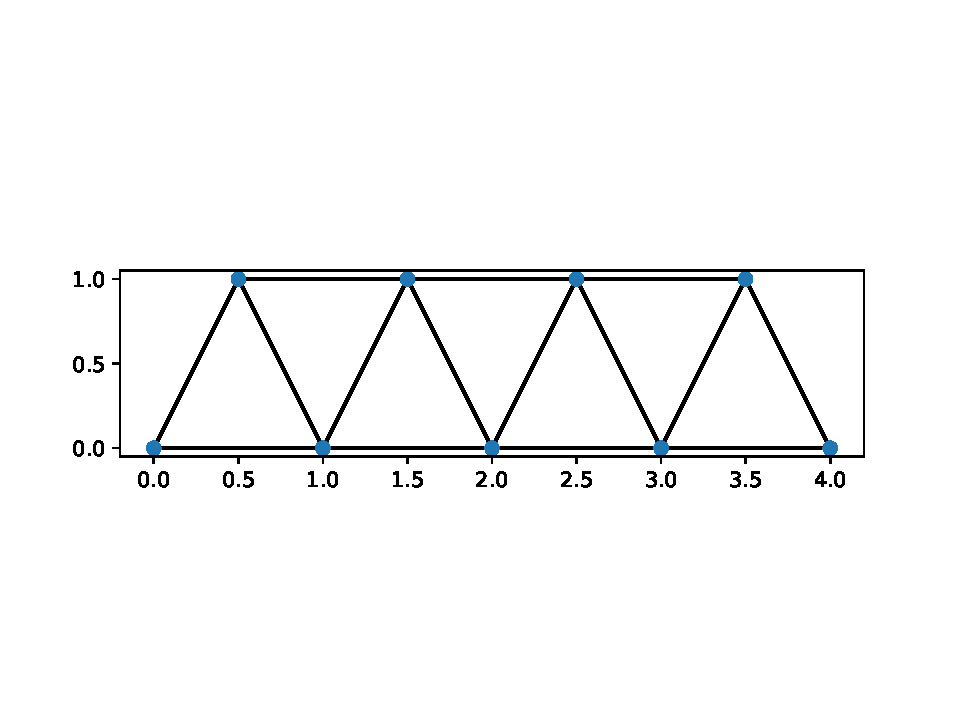
\includegraphics{truss_files/figure-latex/unnamed-chunk-1-1.pdf}

\begin{minted}[autogobble]{python}
dofs = points.size
S = np.zeros((dofs, dofs))
RHS = np.zeros(dofs)

for el in elements:
    local_dof = np.array([2*el['i1'], 2*el['i1']+1, 2*el['i2'], 2*el['i2']+1])
    n = points[el['i2']] - points[el['i1']]
    L = np.sqrt(n.dot(n))
    n = n / L
    N = np.array([[-n[0], -n[1], n[0], n[1]]])
    local_S = np.dot(N.T, np.dot(A*E/L, N))
    S[np.ix_(local_dof, local_dof)] += local_S
    local_load = np.array([0, -0.5, 0, -0.5]) * g * A * L * rho
    RHS[local_dof] += local_load

total_weight = np.sum(RHS)

plt.imshow(S)
plt.show()
\end{minted}

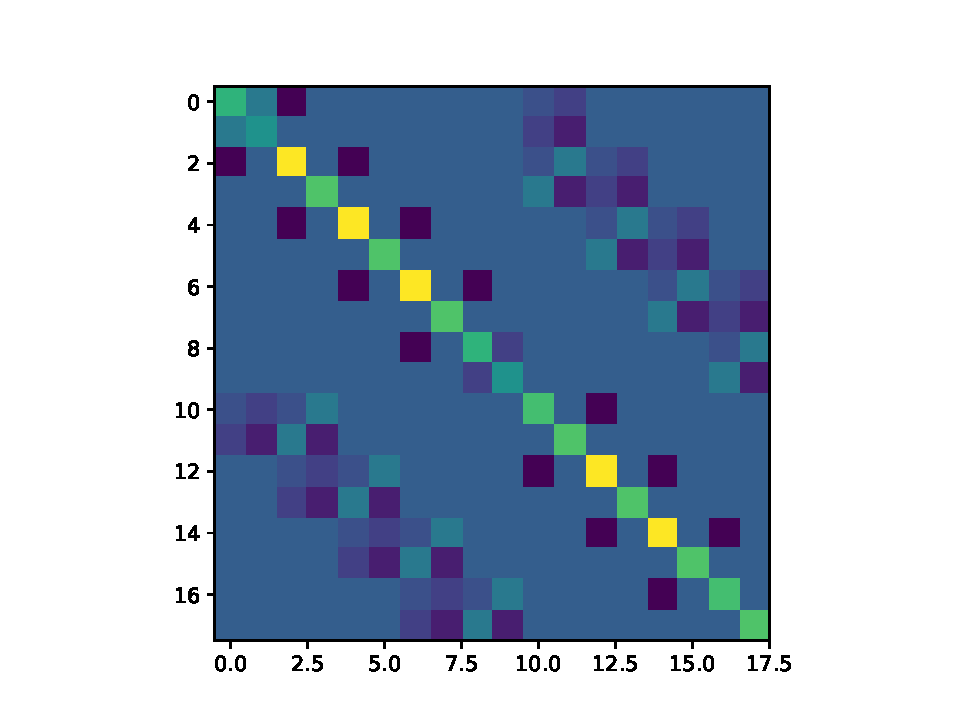
\includegraphics{truss_files/figure-latex/unnamed-chunk-1-2.pdf}

\begin{minted}[autogobble]{python}
to_load = np.array([2*2+1])
load = -1e3 * g  # 1 tonne
RHS[to_load] = load

to_fix = np.array([2*0+0, 2*0+1, 2*4+0, 2*4+1])
S[to_fix, :] = np.eye(dofs)[to_fix, :]
RHS[to_fix] = 0

x = np.linalg.solve(S, RHS)
displacement = np.reshape(x, points.shape)

scale = 10000
plot_beams(points + scale * displacement, elements)
\end{minted}

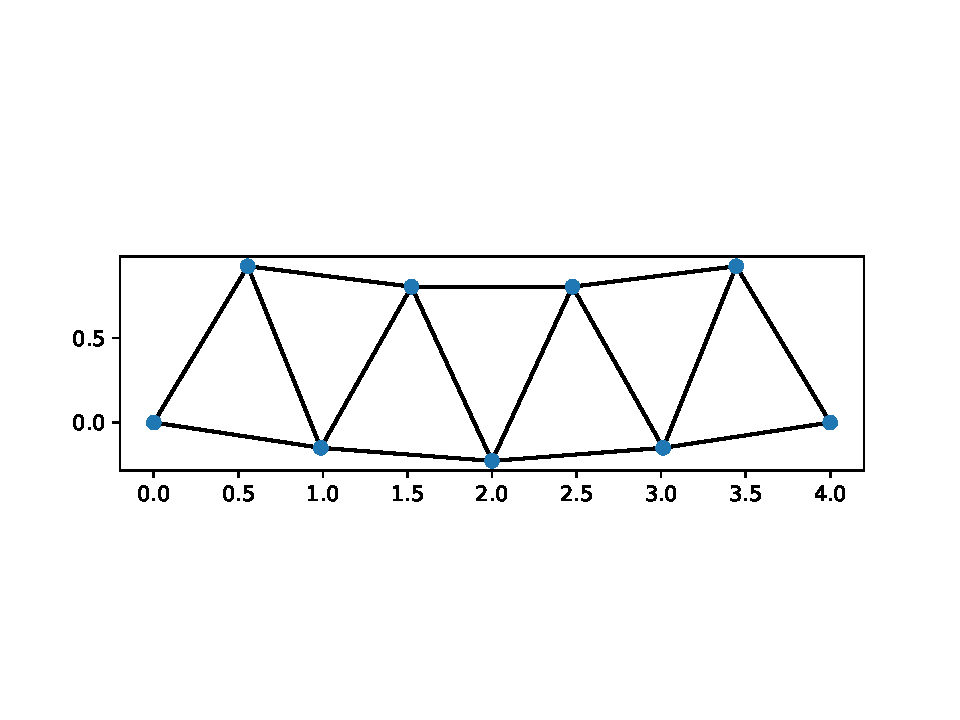
\includegraphics{truss_files/figure-latex/unnamed-chunk-1-3.pdf}


\section{Lecture}
\subsection{FEM as a general method}
For electric current: $I = \frac{1}{R}(V_1-V_0)$, so:
\[\mattwo{\frac{1}{R}}{-\frac{1}{R}}{-\frac{1}{R}}{\frac{1}{R}}\vectwo{V_0}{V_1}=\vectwo{I_0}{I_1}\]
For heat exchange: $Q = \lambda(T_1-T_0)$, so:
\[\mattwo{\lambda}{-\lambda}{-\lambda}{\lambda}\vectwo{T_0}{T_1}=\vectwo{Q_0}{Q_1}\]

Let us consider a rod of length $L$ and non-uniform cross-section $A$ and conductivity $\alpha$. Let us divide it into $n$ elements, each with cross-section $A_i$. We have:
\[\mat{k_1 & -k_1 & 0 & \cdot & 0\\
-k_1 & k_1+k_2 & -k_2 &  \cdots & 0\\
0 & -k_2 & k_2+k_3 & \cdots & 0\\
\cdots\\
0 & 0 & 0 & \cdots & k_n}\mat{T_0\\T_1\\T_2\\\cdots\\T_n} = \mat{0\\0\\0\\\cdots\\0}\]
where $k_i=\frac{A_i\alpha}{l}$ and $l=\frac{L}{n}$. In each element we see a balance of:
\[-k_iT_{i-1}+(k_i+k_{i+1})T_{i}-k_{i+1}T_{i+1} = 0\]
which we can rearrange into:
\[A_i\alpha\frac{T_{i}-T_{i-1}}{l}-A_{i+1}\alpha\frac{T_{i+1}-T_{i}}{l} = 0\]
Which (divided by $l$) one can recognise as a finite difference scheme for:
\[\frac{d}{dx}\left(A\alpha\frac{d}{dx}T\right)=0\]

Question is, how to generalise it?
\subsection{The weak variational form}
Commonly, two main things come into play when considering a numerical method. One is how do we represent our solution, depending on some coefficients, and second is how do we ``check`` if out equation is satisfied.

Let us assume that temperature is linear between the nodes. This can be expressed as:
\[T(x) = \sum_k T_k\phi_k(x)\]
where $\phi_k$ are so-called hat functions (drawing). This is our representation of the solution. In a general case $\phi_i$ can be complex are called shape functions. Now the question is, how to ``check`` if the equation is satisfied. One way would be to evaluate the equation ($\frac{d}{dx}\left(A\alpha\frac{d}{dx}T\right)=0$) in some points. For example middles of the elements. Yet this does not work, as for a linear function (inside of element) this is always satisfied.

What we do in Finite Element Method, is multiply the equation by the same shape functions that were used for representation, and integrate over the domain:
\[\int_\Omega\phi_j\frac{d}{dx}\left(A\alpha\frac{d}{dx}T\right)dx = 0\]

For many representations (eg. our representation) this cannot be integrated. We use the Green-Gauss-Ostrogradsky theorem to reduce the order of derivatives (we will now omit border contribution:
\[\int_{\partial\Omega}[\cdots]-\int_\Omega\left(\frac{d}{dx}\phi_j\right)\left(A\alpha\frac{d}{dx}T\right)dx = 0\]

Such form of the equation, is sometimes called in mathematics the weak form. This is because it requires less of the solution. In reality it should not be considered a `lesser` form of the equation, as most equations used in physics are in fact satisfied in the integral form, as they express conservation laws.

Now, if we substitute our representation we get:
\begin{align*}
-\int_\Omega\left(\frac{d}{dx}\phi_j\right)\left(A\alpha\frac{d}{dx}T\right)dx &= -\int_\Omega\left(\frac{d}{dx}\phi_j\right)\left(A\alpha\frac{d}{dx}\left(\sum_kT_k\phi_k(x)\right)\right)dx =\\
&= -\sum_k\left[\int_\Omega A\alpha\frac{d\phi_j}{dx}\frac{d\phi_k}{dx}dx\right]T_k 
\end{align*}
resulting in a matrix-times-vector form.

Although this form looks, like the elements of the matrix are some general expressions, one should consider them still in the context of the elements. If $\Delta_i$ is the element between $x_{i-1}$ and $x_i$, then:
\[-\int_{\Delta_i} A\alpha\frac{d\phi_j}{dx}\frac{d\phi_i}{dx}dx\]
is non-zero only if both $j$ and $k$ are either $i-1$ or $i$. Moreover the hat functions $\phi$ are linear on the elements, and their derivatives are fixed, and equal to $\pm\frac{1}{l}$. This gives us the same local stiffness matrix as previously:
\[\mat{ & \cdots & \cdots & \\
\cdots & \frac{A_i\alpha}{l} & -\frac{A_i\alpha}{l} & \cdots \\
\cdots & -\frac{A_i\alpha}{l} & \frac{A_i\alpha}{l} & \cdots \\
 & \cdots & \cdots & }\mat{\cdots\\T_{i-1}\\T_i\\\cdots}\]

\subsection{Polynomial element shape functions}

This formulation is very general and allows to discretise many different equations. Let us now write it in a more formal way.

Let us have an equation in 2D:
\[\dive{\left(\alpha\grad{T}\right)} = \pr{x}\left(\alpha\pr{x}T\right) + \pr{y}\left(\alpha\pr{y}T\right) = q\]
Of which the full weak form is:
\[\int_{\partial\Omega}\alpha\psi\pr{n}T-\int_\Omega\alpha\left(\rr{\psi}{x}\rr{T}{x} + \rr{\psi}{y}\rr{T}{y}\right) = \int_\Omega\psi q,\quad\text{for any test function }\psi\]

Now, for the representation $T(x)=\sum_k T_k\phi_k(x)$, and $q(x)=\sum_k q_k\phi_k(x)$:
\[\sum_k\left[\int_{\partial\Omega}\alpha\phi_j\rr{\phi_k}{n}\right]T_k-\sum_k\left[\int_\Omega\alpha\left(\rr{\phi_j}{x}\rr{\phi_k}{x} + \rr{\phi_j}{y}\rr{\phi_k}{y}\right)\right]T_k = \sum_k\left[\int_\Omega\phi_j\phi_k\right]q_k\]

Note that this formulation is not dependent on $\phi_i$ functions being hat functions, linear on elements, or even related to elements. Nevertheless, it is extremely important to keep the number of non-zero elements in used matrices low. Finite element method uses low-order polynomial function across simple elements, to allow for easy computation of needed integrals. (High order polynomials are used in Spectral Element Method.)

As previously noted it is important to consider these expressions in the context of single elements. In these element local element matrices have to be constructed by calculation of relevant integrals.

In most solvers this is done by transformation of the physical coordinates (eg. $x$, $y$) into element coordinate system (eg. $\zeta$, $\eta$) in which the element is always of the same shape (drawings) --- so called, base element.

For $J = \mat{\rr{x}{\zeta} & \rr{x}{\eta}\\\rr{y}{\zeta} & \rr{y}{\eta}}$, we have: $\mat{\rr{f}{x}&\rr{f}{y}}J = \mat{\rr{f}{\zeta}&\rr{f}{\eta}}$. If we assume the transformation is linear (the element in the physical space is a linearly transformed base element) we get:
\newcommand{\baseelementint}[2]{\int_{\Delta}\alpha\rr{\phi_j}{#1}\rr{\phi_k}{#2}}
\begin{align*}    
\int_{\Delta_i}\alpha\left(\rr{\phi_j}{x}\rr{\phi_k}{x} + \rr{\phi_j}{y}\rr{\phi_k}{y}\right) &= \int_{\Delta}\alpha\left(\mat{\rr{\phi_j}{\zeta}&\rr{\phi_j}{\eta}}J^{-1}J^{-T}\mat{\rr{\phi_k}{\zeta}&\rr{\phi_k}{\eta}}^T\right)|J| =\\
&= \left[J^{-1}J^{-T}|J|\right]:\mat{\baseelementint{\zeta}{\zeta} & \baseelementint{\zeta}{\eta} \\ \baseelementint{\eta}{\zeta} & \baseelementint{\eta}{\eta}}\\
\int_{\Delta_i}\phi_j\phi_k &= |J|\int_{\Delta}\phi_j\phi_k
\end{align*}
Which looks more complicated, but one has to remember that the integrals how, can be precomputed, as the base element is constant.

For triangle element in 2D for example we have element matrices:
\begin{align*}
    S &= |J|\mat{-1&1&0\\-1&0&1}^T(J^TJ)^{-1}\mat{-1&1&0\\-1&0&1}\\
    M &= |J|\frac{1}{24}\mat{2&1&1\\1&2&1\\1&1&2}\\
\end{align*}
If time permits, a long rumbling about transformation of scalar product and invariance of physics operators.

\subsection*{Exercises}

\begin{exercise}
For a element size $h$ and four points $p^0=\{0,0\}$, $p^1=\{h,0\}$, $p^2=\{0,h\}$, $p^3=\{h,h\}$ forming a square in 2D:
\begin{enumerate}[label=\alph*)]
\item check what is the minimal order of a polynomial, which could would evaluate to one on one of the points and zero on remaining three.
\item propose four such functions $\phi_i$, each evaluating to one on the corresponding point $p_i$.
\item Compute $\int_\square\phi_i\phi_j$ for every pair of $i$ and $j$. Are there any symmetries you can exploit?
\item Compute $\int_\square \left(\rr{\phi_i}{x}\rr{\phi_j}{x} + \rr{\phi_i}{y}\rr{\phi_j}{y}\right)$
\end{enumerate}
\end{exercise}

\begin{exercise}
For a function $A:\mathbb{R}^{n\times n}\rightarrow\mathbb{R}^{n\times n}$ which takes a matrix and returns a matrix:
\[A(B) = \alpha B + \beta I \tr{B},\quad\text{(reminder: $\tr{B}=\sum_iB_{ii}$)}\]
show that for any matrix $C$:
\[C^{-1}A(B)C = A\big(C^{-1}BC\big)\]
\end{exercise}

\begin{exercise}
For a function $f(x) = e^{\mathrm{i}kx}$ calculate:
\begin{enumerate}[label=\alph*)]
\item $f''(x)$
\item $\frac{2f(x)-f(x+h)-f(x-h)}{h^2}$
\end{enumerate}
And compare the results. What can you say about these results for $f(x) = e^{-\mathrm{i}kx}$ and $f(x) = \cos{kx}$?
\end{exercise}


\subsection*{Contact}
\begin{itemize}
    \item Heat equation on an unstructured mesh
    \item Python implementation/demonstration
\end{itemize}
\begin{minted}[autogobble]{python}
import numpy as np
import matplotlib.pyplot as plt
from mpl_toolkits.mplot3d import Axes3D

Lx = 2
Ly = 1
H = 0.001  # 1mm
nx = 21
ny = 10
alpha = 111e-6  # 111mm^/s

x_vals = np.linspace(0, Lx, nx)
y_vals = np.linspace(0, Ly, ny)
points = np.array(np.meshgrid(x_vals, y_vals, indexing="ij")).T.reshape(-1, 2)
n = points.shape[0]
i0 = np.where((points[:, 0] != Lx) & (points[:, 1] != Ly))[0]  # 0-index
elements = np.array([[i0,i0],[i0 + 1, i0 + nx + 1],[i0 + nx + 1, i0 + nx]]).T.reshape(-1, 3)
m = elements.shape[0]
element_h = np.repeat(H,m)
element_centers = (points[elements[:, 0],:] + points[elements[:, 1],:]+points[elements[:, 2],:]) / 3

sel = (element_centers[:,0] > Lx * 0.3) & (element_centers[:,0] < Lx * 0.7) & (element_centers[:,1] > Ly * 0.5)
element_h[sel] = H / 10

plt.tripcolor(points[:,0],points[:,1],elements,facecolors=element_h)
plt.show()
\end{minted}

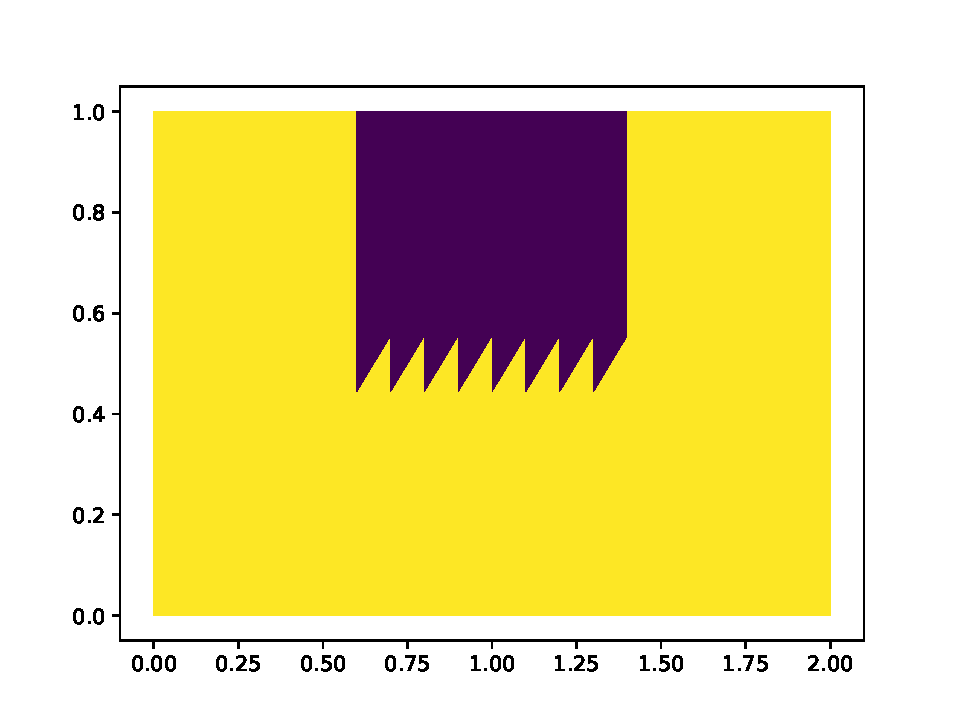
\includegraphics{heat_files/figure-latex/unnamed-chunk-1-1.pdf}

\begin{minted}[autogobble]{python}
dofs = n
RHS = np.zeros(dofs)
S = np.zeros((dofs, dofs))
M = np.zeros((dofs, dofs))

for el, h in zip(elements, element_h):
    J = np.array([points[el[1],:]-points[el[0],:],points[el[2],:]-points[el[0],:]])
    local_dof = el
    tmp1 = np.linalg.det(J) * np.linalg.inv(np.dot(J.T, J))
    tmp2 = np.array([[-1, 1, 0], [-1, 0, 1]])
    local_S = np.dot(np.dot(tmp2.T, tmp1), tmp2) * h * alpha
    S[np.ix_(local_dof, local_dof)] += local_S
    local_M = np.linalg.det(J) * np.array([[2, 1, 1], [1, 2, 1], [1, 1, 2]]) / 24
    M[np.ix_(local_dof, local_dof)] += local_M

plt.imshow(S)
plt.show()
\end{minted}

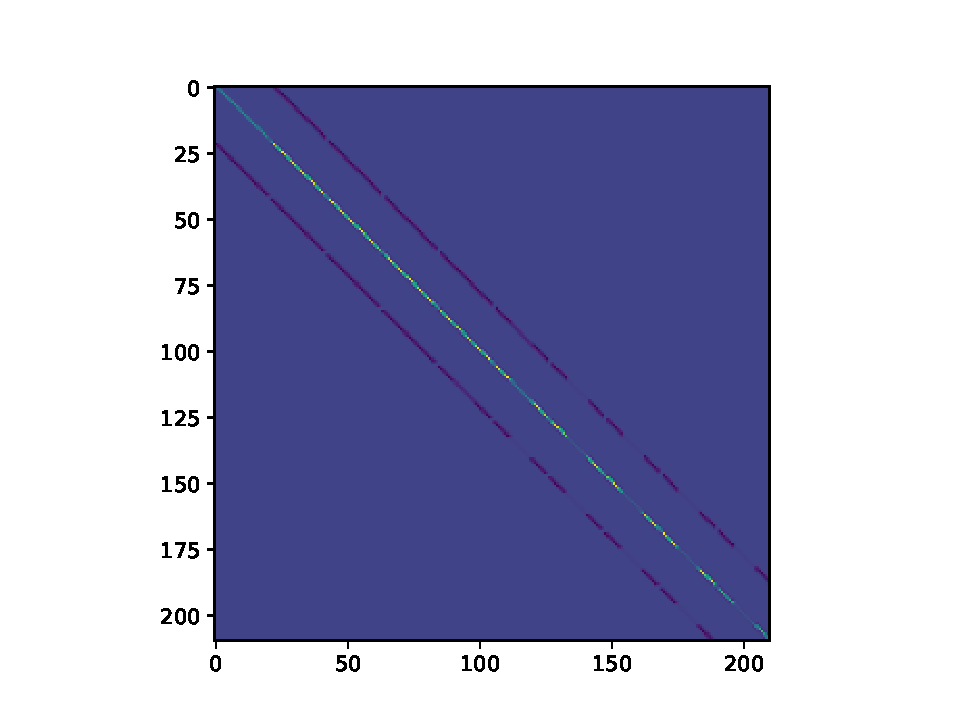
\includegraphics{heat_files/figure-latex/unnamed-chunk-1-2.pdf}

\begin{minted}[autogobble]{python}
plt.imshow(M)
plt.show()
\end{minted}

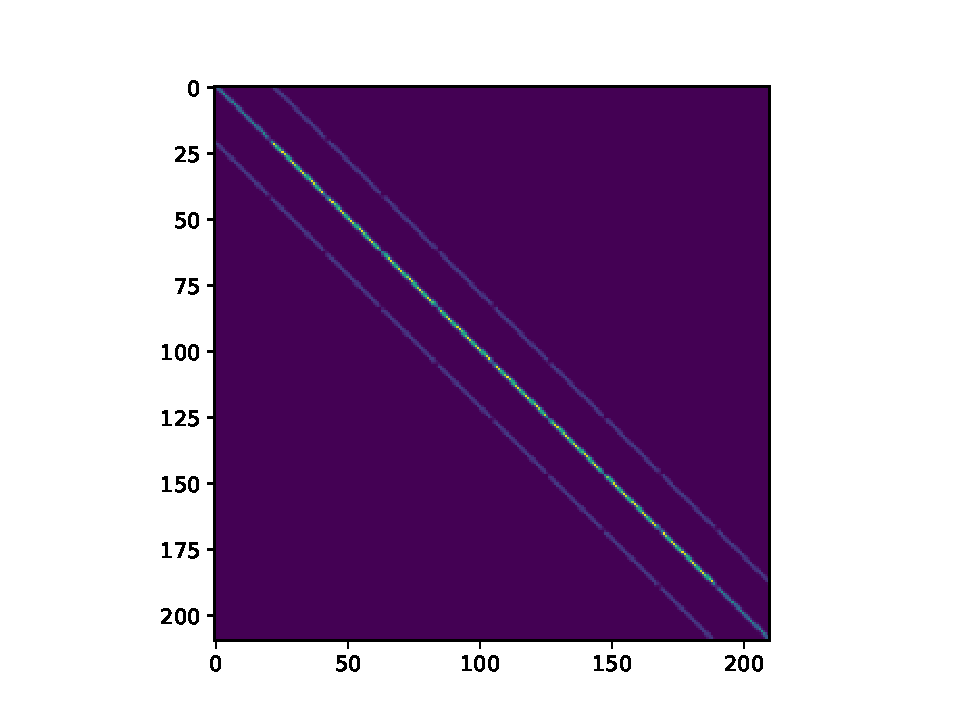
\includegraphics{heat_files/figure-latex/unnamed-chunk-1-3.pdf}

\begin{minted}[autogobble]{python}
to_fix = np.where(points[:, 0] == 0)[0]
S[to_fix, :] = np.eye(dofs)[to_fix, :]
RHS[to_fix] = 1

to_fix = np.where(points[:, 0] == Lx)[0]
S[to_fix, :] = np.eye(dofs)[to_fix, :]
RHS[to_fix] = 0

x = np.linalg.solve(S, RHS)

plt.tripcolor(points[:,0],points[:,1],elements,x,shading='gouraud')
plt.show()
\end{minted}

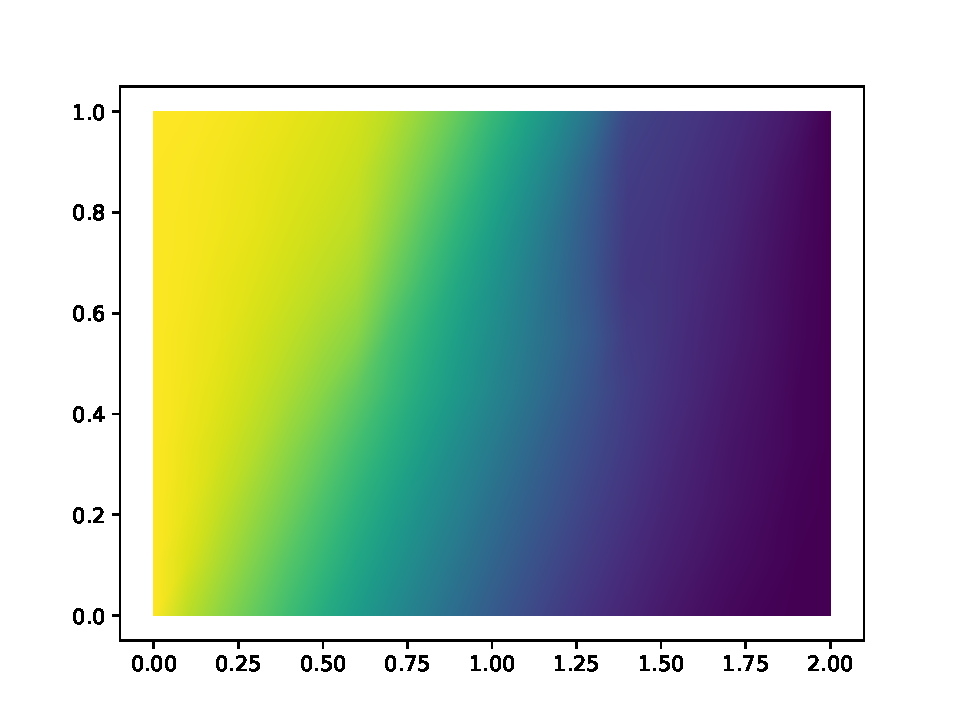
\includegraphics{heat_files/figure-latex/unnamed-chunk-1-4.pdf}


\section{Lecture}
\subsection{Mechanics of linear elastic materials}
If we look at the force relation for the beam:
\[\frac{AE}{L}x=F\]
We can rearrange it to get:
\[E\underbrace{\frac{x}{L}}_\text{strain}=\underbrace{\frac{F}{A}}_\text{stress}\]
Notice now that there is some strain in the y and z directions. This is because the rod ``expands`` in these directions. This expansion is quantified with the Poisson ratio: $\frac{y}{D} = \nu\frac{x}{L}$. 

In real applications, stress is a more complex state than a single number (scalar) or even a vector. Let us imagine some metal part under load. Let us now imagine a small incision inside of the metal. Will it be pulled apart? will it be squashed? Will the two sides slide with respect to each other?

\newcommand{\pforce}{\overrightarrow{p}}
For a given direction $n$ we can imagine a small square normal to his vector. The force acting on this square divided by the area of the square in a vector $\pforce$. In fact this square is not moving anywhere, so the metal on one side is acting on it with force $\pforce$, and the metal on the opposite side is acting with force $-\pforce$. It is a matter of convention which $\pforce$ to take, but standard way is to take the one acting from the side in which $n$ is pointing.

\fbox{Stress tensor (or matrix) is defined as $\sigma$, so that $\pforce(n) = \sigma\cdot n$ for all directions.}

One can think of this quantity, as a ``thing`` that takes a direction and gives you a force acting between ``layers`` of the material in this direction.

If we have a piece of the part $\Omega$, we can calculate the total force acting on in from all sides ($\partial\Omega$) by integration:
\[F = \int_{\partial\Omega} \sigma\cdot n\]

From the Green-Gauss-Ostrogradsky theorem, we have: $F = \int_{\partial\Omega} \sigma n = \int_{\Omega} \dive\sigma $. Finally, in the equlibrium state nothing is moving, so this $F$ plus any external load $f$ is equal to zero for any $\Omega$. This means that:
\[\dive\sigma + f = 0\quad\text{which means: }\sum_i\pr{x_i}\sigma_{ij} + f_j = 0\]

This gives us our main conservation equation of solid mechanics: divergence of stress is equal to load. Now the question that is left is how the stress depends on the deformation.

Let us have a displacement field $u(x)$. We can make several simplifying assumptions about the dependence of $\sigma$ on $u$, in the order of least to most restrictive:
\begin{enumerate}
    \item the dependence is invariant to translation and rotation of the object
    \item pure translation and rotation do not produce any stress in the material.
    \item $\sigma$ in a point $x$ depends only on the displacements in the immediate vicinity of the point.
    \item $\sigma$ depends only on the first derivatives of $u$
    \item $\sigma$ is a linear function of first derivatives of $u$
\end{enumerate}
Resulting model is the so-called assumption of linear elasticity. If we additionally assume the material to be isotropic, the only form of the dependence, which satisfies all these criteria is:
\[\sigma_{ij} = \mu\left(\rr{u_i}{x_j}+\rr{u_j}{x_i}\right) + \lambda\delta_{ij}\sum_k\rr{u_k}{x_k}\]
for some coefficients $\lambda$ and $\mu$, called (the first and second) Lam\'e parameters. The expression in brackets is the so-called symmetric gradient of $u$:
\[\varepsilon_{ij} = \frac{1}{2}\left(\rr{u_i}{x_j}+\rr{u_j}{x_i}\right)\]
and in the context of the linear elasticity theory is called the infinitesimal strain tensor (Strain has different definitions depending on the context). This gives the most common form of the constitutive equation of isotropic linear media:
\[\sigma = 2\mu\varepsilon + \lambda I \tr{\varepsilon}\]

The Lam\'e parameters, can be tied to the more commonly used Young's modulus $E$, and Poisson's ratio $\nu$:
\[\lambda = \frac{E\nu}{(1+\nu)(1-2\nu)}\quad\text{and}\quad\mu=\frac{E}{2(1+\nu)}\]

\subsection{Plane stress/strain, uniaxial/biaxial loading, shear}

Strain and stress can have reduced dimensionality when confined to 2D or 1D cases. Nevertheless it is vital to understand that the presence of first Lam\'e parameter (or Poisson's ration) means that strain in any direction contributes to any direction of stress, and vice-versa. This means that even if we have no stress in one direction (so-called plane stress):
\[\sigma=\mat{
\sigma_{xx}&\sigma_{xy}&0\\
\sigma_{yx}&\sigma_{yy}&0\\
0&0&0}\]
the strain can still have components in all directions. An opposite situation is called plane strain. Similarly, one can have single direction stress tensor (as in loaded beam), and one-directional strain.

To understand when these situations occur, the simplest is to remember that zero-strain (in any direction) occurs when material cannot expand or contract in this direction. For instance if it is in a large bulk of material in said direction. Whereas zero stress in most cases corresponds to material not being constraint or loaded in this direction.
\begin{itemize}
    \item axially loaded beam
    \item tensioned membrane
    \item beam loaded from sides
    \item compressed underground rock
    \item bending of a beam
    \item wall of pressure tank (trick question)
\end{itemize}

These regimes can be simulated in 2D and 1D respectively, but one has to use the right one.

\subsection{Element technology (e.g. solids, shells, membranes, beams)}

One can derive Finite Element Method for the elastic medium, by either discretising the $\dive\sigma=f$ equation, or integrating the elastic energy $\frac{1}{2}\sigma:\epsilon$ over the element.

Commonly used elements to divide the interior of structures are simple polyhedra with displacement degrees of freedom in vertices, or less commonly in middles of edges or faces.

It is common to neglect one or two dimensions of the elements assuming a simplified forms of displacement and stress in these directions. This simplified state is frequently encoded by additional degrees of freedom, like rotation.

TODO: beam element types, membranes and RBE2 and RBE3.

\subsection*{Exercises}
\begin{exercise}
    Show that stress tensor $\sigma$ is symmetric, by assuming $\sigma$ is constant in a region and calculating the moment acting on a small rectangular prism.
\end{exercise}

\begin{exercise}
Show that $\lambda = \frac{E\nu}{(1+\nu)(1-2\nu)}$ and $\mu=\frac{E}{2(1+\nu)}$, by substituting the stress and strain in a axially loaded beam into the constitutive equation.
\end{exercise}

\begin{exercise}
TODO
\end{exercise}

\subsection*{Contact}
\begin{itemize}
    \item Ansys demonstration
    \item Structures with solid and shells
    \item Post-processing and visualisation
\end{itemize}
\section{Lecture}
\subsection{Workflow revisited --- Preparation of geometry}
At this stage it is crucial to consider how the physical case can be simplified to preserve the desired physics, but simplify the computation. This is not only because we want to save time on the computation itself, but because (as a rule) simpler setups are less prone to cause you problems along the way.

Examples of simplifications:
\begin{itemize}
    \item 2D vs 3D
    \item Dimension reduction of beams, frames, plates and shells
    \item Removing non-crucial features, bevel/chamfer/fillets, threads, holes, rivets, etc. If they are not to be resolved.
    \item Symmetries (including axial-symmetry)
    \item Periodicity (especially rotational)
\end{itemize}

Another thing to remember is that the final geometry has to be, 1. good quality for meshing, and 2. have well defined features for setting up boundary conditions.

\subsection{Workflow revisited --- Meshing}
In most cases, meshing for FEM structural analysis is not a challenging problem for modern software. This is not the case for CFD, which will be obvious in the later part of the course. Nevertheless, frequently getting {\it any} mesh is easy, but getting a {\it good} mesh is hard.

It is good to remind outselves that the computer is just very quickly doing the analysis we did in previous lectures. Including computing some integrals, and crucially, changes of variables between the physical space, and the idealised element space. As one can imagine, the harder it is to invert the Jacobian matrix of this transform, the more prone to error are these computations. How a matrix is hard to invert is frequently measured by the conditional number, which is the ratio of the biggest eigenvalue to the smallest. But there are simpler, more intuitive measures of how ``bad`` is this trasform.
\begin{itemize}
    \item Aspect ratio
    \item Various measures of angles in elements (maximal angle between edges) or between elements (angle between center-to-center segment and face normal direction)
\end{itemize}
In most cases the best way to get good quality mesh is to generate a so-called block structure mesh.

Describe:
\begin{itemize}
    \item 2D meshing
    \item Extrusion
    \item O-type mesh
    \item C-type mesh
\end{itemize}

\subsection{Workflow revisited --- Simulation setup}
The most important thing about simulation setup is (again) simplification. If one can make certain assumptions, or ignore some effects, it should be done. The same reasoning applies: not only it will make the simulation cheaper, but will reduce the probability of unforeseen problems.

Examples of this include calculating 1D beam versus 3D meshed beam, or calculating compressible flow for a nearly in-compressible regime.

Examples of simplifications:
\begin{itemize}
    \item Plane stress/strain
    \item Calculating in linear regime
    \item Calculating only small deformations
    \item Simplification of loads (inc. pressure)
\end{itemize}

At this stage one has to carefully consider applied boundary conditions, such as:
\begin{itemize}
    \item Zero displacement and/or rotation
    \item Fixed displacement
    \item Zero normal stress
    \item Symmetry and periodicity
    \item Mixed conditions (explain reduced representations)
\end{itemize}

\subsection{Workflow revisited --- Computation}
Modern software can efficiently use multi-core architectures, but scaling is not always perfect. Explain about code scaling and mechanism for parallelisation. Explain the common ways to use HPC systems.

It is important to monitor convergence measures. Moreover one has to remember that the conducted simulation is just one realisation of the setup. One of the most obvious signs of trouble is when the solution is very sensitive to the setup or the mesh.

Discuss mesh convergence, and pitfalls.

\subsection{Workflow revisited --- Post-processing and analysis}
First and foremost goal of post-processing should be {\bf verification} of the assumptions made during all previous steps, and verification of the method itself.

Sometimes this can be as simple as checking if the assumed small deformations in linear regime, are really small and in the linear regime. Sometimes however it is a hard task, as for example: a assumed symmetry will force the solution to be symmetric, even if the ``real`` solution is not. This can be sometimes caught by detailed inspection of the results and convergence.

Most of the mesh quality inspection should be done before computation, but at the post-processing stage one should also inspect if mesh is detailed enough to represent the computed physical features. If not, frequently zig-zag patterns will occur or values of fields will ``unnaturally` jump across elements.

{\bf Comparison with hand-calculated approximate values is always a good idea.} It can catch order-of-magnitude errors, bad boundary conditions, wrong load directions, and many more.

\begin{center}\fbox{Get excited about your results, only after you verified that your simulation is right.}\end{center}

In most structural analysis, there are two properties one is interested in:
\begin{itemize}
    \item Stress/strain fields in the bulk of the domain. Especially maximums of selected stress criteria (eg. von Mises yield criterion)
    \item Displacement in specific points.
\end{itemize}

\subsection{Workflow revisited --- Design improvement}

\subsection*{Exercises}
\begin{exercise}
    Write the form of the stress and strain matrices on the symmetry plane (assume the symmetry is in $z$ direction)
\end{exercise}
\begin{exercise}
    TODO
\end{exercise}

\subsection*{Contact}
\begin{itemize}
    \item Ansys meshing demonstration
    \item Measures of element quality
    \item Grid convergence analysis
\end{itemize}

\section{Lecture}
\subsection{Solution methods}
Direct and iterative methods. Pro`s and con`s, plus comment on conjugate gradient.
\subsection{Dynamics and vibration}

\begin{center}
\begin{circuitikz}
\node[draw, rounded corners=2pt,inner sep=10pt] (mass1) at (3,0) {$M_1$};
\node[draw, rounded corners=2pt,inner sep=10pt] (mass2) at (6,0) {$M_2$};
\draw 
(0,0) to[R={$k$},-] (mass1.west)
(mass1.east) to[R={$k$},-] (mass2.west);
\draw (0,-0.5) -- (0,0.5);
\end{circuitikz}
\end{center}
\newcommand{\gr}{\color{gray}}
\[\mat{\gr 0 & \gr 0 & \gr 0\\ \gr 0 & M_1&0\\\gr 0 &0&M_2}\mat{\gr 0\\\ddot{x_1}\\\ddot{x_2}} + \mat{\gr k & \gr-k & \gr 0\\\gr -k & k+k & -k\\\gr 0 &-k&k}\mat{\gr 0\\x_1\\x_2} = \mat{\gr 0\\F_1\\F_2}\]

\[\mat{\gr 0 & \gr 0 & \gr 0\\ \gr 0 & M_1&0\\\gr 0 &0&M_2}\mat{\gr 0\\\ddot{x_1}\\\ddot{x_2}} + \mat{\gr c & \gr-c & \gr 0\\\gr -c & c+c & -c\\\gr 0 &-c&c}\mat{\gr 0\\\dot{x_1}\\\dot{x_2}} + \mat{\gr k & \gr-k & \gr 0\\\gr -k & k+k & -k\\\gr 0 &-k&k}\mat{\gr 0\\x_1\\x_2} = \mat{\gr 0\\F_1\\F_2}\]

In general:
\[M\ddot x + D\dot x + Sx = F\]

\begin{align*}
\frac{d}{dt} E
&= \frac{d}{dt}\left(\frac12\dot x^TM\dot x + \frac12 x^TSx + x^TF\right) =\\
&= \dot x^TM\ddot x + \dot x^TS x + \dot x^TF =\\
&= \dot x^T\left(M\ddot x + S x + F\right) =\\
&= \dot x^T\left(M\ddot x + D\dot x + S x + F\right) - \dot x^TD\dot x =\\
&= - \dot x^TD\dot x
\end{align*}

Generalized eigenvalue problem $Sv^i = \lambda_i Mv^i$ which in full form is:
\[SV = MV\Lambda\quad\text{where}\quad V^TMV=I\]
for $x = V\beta$, and $D=\alpha_1M+\alpha_2S$, we have:
\[MV\ddot\beta + (\alpha_1M+\alpha_2S)V\dot\beta + SV\beta = F\]
Using generalised eigenvalue equation,
\[MV\ddot\beta + (\alpha_1MV+\alpha_2MV\Lambda)\dot\beta + MV\Lambda\beta = F\]
and multiplying by $V^T$,
\[\ddot\beta + (\alpha_1+\alpha_2\Lambda)\dot\beta + \Lambda\beta = V^TF\]
we get complete separation of equations:
\[\ddot\beta_i + (\alpha_1+\alpha_2\lambda_i)\dot\beta_i + \lambda_i\beta_i = v^i\cdot F\]


\subsection{Implicit vs explicit techniques}
\[\begin{cases}
M\dot y &= F - Dy - Sx\\
\dot x &= y
\end{cases}\]

A fully explicit scheme:
\[\begin{cases}
M y_{n+1} &= M\dot y_n + dt(F - Dy_n - Sx_n)\\
x_{n+1} &= x_n + dt y_n
\end{cases}\]


Half-implicit (TODO: correct to be leapfrog):
\[\begin{cases}
M y_{n+1} &= M\dot y_n + dt(F - Dy_n - Sx_n)\\
x_{n+1} &= x_n + dt y_{n+1}
\end{cases}\]

Implicit:
\[\begin{cases}
M y_{n+1} &= M\dot y_n + dt(F - Dy_{n+1} - Sx_{n+1})\\
x_{n+1} &= x_n + dt y_{n+1}
\end{cases}\]


\subsection*{Exercises}
\begin{exercise}
    Show that without dumping, energy in the explicit method is constatly growing, and constantly decreasing in implicit method. 
\end{exercise}

\begin{align*}
E_{n+1} 
&= \frac12 y_{n+1}^TMy_{n+1} + \frac12 x_{n+1}^TSx_{n+1} + x_{n+1}^TF =\\
&= \frac12 \left(M\dot y_n + dt(F - Dy_n - Sx_n)\right)^TM^{-1}\left(M\dot y_n + dt(F - Dy_n - Sx_n)\right) + \frac12 \left(x_n + dt y_n\right)^TS\left(x_n + dt y_n\right) + \left(x_n + dt y_n\right)^TF =\\
&= \frac12 y_n^TMy_n + dty_n^T\left(F - Dy_n - Sx_n\right) + \frac12dt^2\left(F - Dy_n - Sx_n\right)^T M^{-1}\left(F - Dy_n - Sx_n\right) + \frac12 x_n^TSx_n + dt y_n^TSx_n + \frac12dt^2y_n^TSy_n + x_n^TF + dt y_n^TF =\\
&= E_n + dt \left[y_n^T\left(F - Dy_n - Sx_n\right) + y_n^TSx_n + y_n^TF\right] + \frac12dt^2\left[\left(F - Dy_n - Sx_n\right)^T M^{-1}\left(F - Dy_n - Sx_n\right) + y_n^TSy_n\right] =\\
&= E_n - dt y_n^TDy_n + \frac12dt^2\left[\left(F - Dy_n - Sx_n\right)^T M^{-1}\left(F - Dy_n - Sx_n\right) + y_n^TSy_n\right] =\\
\end{align*}


\subsection*{Contact}
\begin{itemize}
\item Ansys worked example
\item Vibration problem (from Helimods)
\item Comparison to loading  frequencies
\end{itemize}

\section{Lecture}
\subsection{Geometric nonlinearity}
\subsection{Hyperelastic and post-elastic materials}
\subsection{Contact problems}
\subsection*{Contact}
\begin{itemize}
    \item Ansys demonstration
    \item Rail isolation system?
\end{itemize}
\end{document}
